\documentclass[defernumbers,nosortbib]{fefu}

\usepackage{bm}
\usepackage{minted}
\usepackage{amssymb}
\usepackage{subfiles}
\usepackage{nicefrac}
\usepackage{subcaption}
\usepackage{placeins}
\usepackage{tabularx}

\setmainfont{CMU Serif}
\addbibresource{../references.bib}
\graphicspath{{../images/}}

\fefuloadstyle[../]{poi_phd}

\newcounter{sectionscount}
\newcounter{allpagescount}
\newcounter{textpagescount}
\newcounter{figurescount}
\newcounter{tablescount}
\newcounter{citescount}
\newcounter{bibpagescount}
\newcommand{\handlecounts}{%
    \input{../counters.tex}%

	\setcounter{sectionscount}{\pgfkeysvalueof{/counters/sectionscount}}%
    \setcounter{allpagescount}{\pgfkeysvalueof{/counters/allpagescount}}%
    \setcounter{textpagescount}{\pgfkeysvalueof{/counters/textpagescount}}%
    \setcounter{figurescount}{\pgfkeysvalueof{/counters/figurescount}}%
    \setcounter{tablescount}{\pgfkeysvalueof{/counters/tablescount}}%
    \setcounter{citescount}{\pgfkeysvalueof{/counters/citescount}}%
    \setcounter{bibpagescount}{\pgfkeysvalueof{/counters/bibpagescount}}%
}

\newcommand{\pa}[1]{\left(#1\right)}
\newcommand{\code}[2][text]{\mintinline{#1}{#2}}
\newcommand{\niceref}[2]{\hyperref[#1]{#2 \ref{#1}}}
\newcommand{\dd}{\mathrm{d}}
\newcommand{\introductiontitle}{Общая характеристика работы}

\makeatletter
\newcommand{\maybeniceref}[3]{
    \@ifundefined{r@#1}{#2 #3}{\niceref{#1}{#2}}
}
\makeatother

\makeatletter
\@FEFUnotoctrue
\titleformat{name=\section,numberless}[block]
{\bfseries\large}{}{0pt}{#1}
\makeatother

\author{Тыщенко Андрей Геннадьевич}
\setfaculty{1.3.7 -- Акустика}
\setsupervisor{Петров Павел Сергеевич}{д.ф.-м.н.}
\title{Численное моделирование распространения широкополосных акустических сигналов в мелком море с использованием модовых параболических уравнений}

\newcolumntype{L}[1]{>{\raggedright\let\newline\\\arraybackslash\hspace{0pt}}p{#1}}
\newcolumntype{B}[1]{>{\raggedright\let\newline\\\arraybackslash\hspace{0pt}}b{#1}}
\newcolumntype{R}[1]{>{\raggedleft\let\newline\\\arraybackslash\hspace{0pt}}b{#1}}

\defbibfilter{mine}{keyword=myarticles or keyword=myproceedings or keyword=myprograms}

\newcommand{\chooseifabstract}[2]{#2}
\newcommand{\chooseifabstracttwo}[2]{#2}

\begin{document}
    \newgeometry{a4paper,left=1.75cm,right=1.75cm,top=2cm,bottom=2cm}
    \fontsize{14}{16}\selectfont
    \thispagestyle{empty}
    \begin{flushright}
        На правах рукописи
        \vspace{2cm}
    \end{flushright}
    \begin{center}
        \setstretch{2}
        \makeatletter
        {\large\@author}\\
        \bigskip
        \bigskip
        \textbf{\Large\@title}\\
        \bigskip
        \bigskip
        \bigskip
        \setstretch{1.5}
        \@FEFUfaculty\\
        \bigskip
        \bigskip
        \setstretch{1.5}
        АВТОРЕФЕРАТ\\
        диссертации на соискание учёной степени\\
        кандидата физико-математических наук
        \vfill\null
        Владивосток -- \the\year
        \makeatother
    \end{center}
    \newpage
    \thispagestyle{empty}
    \begin{center}
        Работа выполнена в Федеральном государственном бюджетном учреждении науки Тихоокеанском океанологическом институте им. В.И. Ильичёва Дальневосточного отделения Российской академии наук (ТОИ ДВО РАН).
    \end{center}
    \noindent\begin{tabular}{@{}L{7cm}L{10cm}@{}}
        \textbf{Научный руководитель:} & \textbf{Петров Павел Сергеевич,}\newline д.ф.-м.н., главный научный сотрудник, лаборатория 3/2 геофизической гидродинамики, ТОИ ДВО РАН\\
        \textbf{Официальные оппоненты:} & \textbf{Цысарь Сергей Алексеевич,}\newline к.ф.-м.н. доцент кафедры нанофотоники физического факультета МГУ им. М.В. Ломоносова\newline\textbf{Вировлянский Анатолий Львович,}\newline д.ф.-м.н. заведующий лабораторией статистических методов в акустике океана, ИПФ РАН\\
        \textbf{Ведущая организация:} & ФГАОУ ВО \guillemotleft Национальный исследовательский университет ИТМО\guillemotright
    \end{tabular}
    \makeatletter
    \vfill
    \par\noindent Защита состоится \@FEFUdate[12.09]{6cm} в \@FEFUfield{13:00}{1cm} на заседании диссертационного совета а 24.1.214.01 при ФГБУН Тихоокеанском океанологическом институте им. В.И. Ильичева по адресу: 690041, г. Владивосток, ул. Балтийская, д. 43.
    \vfill
    \par\noindent С диссертацией можно ознакомиться в библиотеке ТОИ ДВО РАН, а также на сайте института по адресу: \@FEFUfield{\url{https://www.poi.dvo.ru/ru/node/2347}}{9cm}.
    \vfill
    \par\noindent Автореферат разослан \@FEFUdate{8cm}
    \vfill
    \par\noindent Отзывы и замечания по автореферату в двух экземплярах, заверенные печатью, просьба высылать по вышеуказанному адресу на имя учёного секретаря диссертационного совета.
    \vfill
    \par\noindent\begin{tabular}{@{}B{10cm}R{7cm}@{}}
        Ученый секретарь диссертационного совета, кандидат технических наук & Костив А.Е.
    \end{tabular}
    \makeatother
    \newpage
	\subfile{../subfiles/introduction.tex}
	\newpage
	\section*{Содержание работы}
	\par\textbf{Во Введении} обоснована актуальность диссертационной работы, сформулирована цель и аргументирована научная новизна исследований, показана
	практическая значимость полученных результатов, представлены выносимые
	на защиту научные положения.
	\par \textbf{В первой главе} приводится краткий обзор некоторых классов задач акустики океана, для решения которых моделирование трёхмерных звуковых полей играет важную роль, в частности рассматриваются задачи акустического мониторинга и дальней акустической навигации. Кратко обсуждаются известные средства моделирования трёхмерных акустических полей и формулируются требования к модели, которая разрабатывается в настоящей диссертации.
	\par \textbf{Вторая глава} посвящена описанию математической части поставленной задачи и методам её решения. В \textbf{разделе 2.1} описывается математическая постановка задачи. Звуковое поле ищется в форме модового разложения
	\begin{equation}
		p\pa{x,y,z}=\sum\limits_{j=1}^\infty A_j\pa{x,y}\varphi_j\pa{z,x,y}\,,
	\end{equation}
	где $A_j\pa{x,y}$ называются модовыми амплитудами и в адиабатическом приближении удовлетворяют уравнению горизонтальной рефракции
	\begin{equation}
		\frac{\partial^2A_j\pa{x,y}}{\partial x^2}+\frac{\partial^2 A_j\pa{x,y}}{\partial y^2}+k_j^2\pa{x,y}A_j\pa{x,y}=-\delta\pa{x}\delta\pa{y}\varphi_j\pa{z_s,0,0}\,,
	\end{equation}
	при этом модовые функции $\varphi_j\pa{z,x,y}$ и соответствующие им волновые числа $k_j\pa{x,y}$ являются решениями соответствующей спектральной задачи при фиксированных $x$ и $y$. Далее в \textbf{разделе 2.2} решение уравнения горизонтальной рефракции сводится к решению псевдодифференциального модового параболического уравнения вида (в приближении однонаправленного распространения)
	\begin{gather}
		A_j\pa{x,y}=e^{ik_{j,0}x}\mathcal{A}_j\pa{x,y}\,,\\
		\frac{\partial\mathcal{A}_j\pa{x,y}}{\partial x}=ik_{j,0}\pa{\sqrt{1+L_j}-1}\mathcal{A}_j\pa{x,y}\,,\label{eq::PDMPE}\\
		k_{j,0}^2L_j=\frac{\partial^2}{\partial y^2}+k_j^2\pa{x,y}-k_{j,0}^,.
	\end{gather}
	\par В \textbf{разделе 2.3} подробно рассматриваются аппроксимация псевдодифференциального оператора и дискретизация уравнения \eqref{eq::PDMPE} по координате $x$ с использованием аппроксимации Паде и метода Split-step Pad\'e (SSP). Последний заключается в формальном решении уравнения на равномерной сетке $\Delta x=h$ в виде
	\begin{equation}
		\mathcal{A}_j^{n+1}=e^{ik_{j,0}h\pa{\sqrt{1+L_j}}}\mathcal{A}_j^n\,.
	\end{equation}
	Затем аппроксимация Паде применяется к операторной экспоненте
	\begin{equation}
		e^{ik_{j,0}h\pa{\sqrt{1+L_j}}}\approx\frac{U_{l,m}\pa{L_j}}{W_{l,m}\pa{L_j}}=a_{l,m}^0+\sum\limits_{i=1}^{p=\max\left\{l,m\right\}}\frac{a_{l,m}^i}{1+b_{l,m}^iL_j}\,.
	\end{equation}
	Далее в \textbf{разделе 2.4} проводится дискретизация оператора $L_j$ на равномерной сетке $\Delta y=\delta$ и приводится численная схема решения уравнения \eqref{eq::PDMPE}
	\begin{gather}\label{eq::numerical_scheme}
		\mathcal{A}_j^{n+1,q}=a_{l,m}^0\mathcal{A}_j^{n,q}+\sum\limits_{i=1}^{p}a_{l,m}^i\mathcal{B}_{j,i}^{n+1,q}\,,\\
		\pa{1+b_{l,m}^iL_j^\delta}\mathcal{B}_{j,i}^{n+1,q}=\mathcal{A}_j^{n,q},\quad i=\overline{1,p}\,,\\
		\underset{\alpha_{j,i}}{\underbrace{\frac{b_{l,m}^i}{k_{j,0}^2\delta^2}}}\mathcal{B}_{j,i}^{n+1,q-1}+\underset{\beta_{j,i}}{\underbrace{\pa{1+\frac{b_{l,m}^i}{k_{j,0}^2}\pa{k_j^2-k_{j,0}^2-\frac{2}{\delta^2}}}}}\mathcal{B}_{j,i}^{n+1,q}+\underset{\gamma_{j,i}}{\underbrace{\frac{b_{l,m}^i}{k_{j,0}^2\delta^2}}}\mathcal{B}_{j,i}^{n+1,q+1}=\mathcal{A}_j^{n,q}\,.
	\end{gather}
    Таким образом решение уравнения может быть получено путём последовательного обращения трёхдиагональных матриц.
	\par В \textbf{разделе 2.5} рассматриваются методы искусственного ограничения расчётной области. В первую очередь рассматривается метод согласованных поглощающих слоёв, заключающийся в расширении вычислительной области на $\varepsilon$ с обеих сторон по координате $y$ и замене оператора $L_j$ на оператор $L_j^{PML}$
    \begin{equation}
        k_{j,0}^2L_j^{PML}=\frac{1}{1+i\beta\pa{y}}\frac{\partial}{\partial y}\frac{1}{1+i\beta\pa{y}}\frac{\partial}{\partial y}+k_j^2+k_{j,0}^2\,,
    \end{equation}
    где $\beta\pa{y}$ -- некоторая гладкая функция, монотонно возрастающая при удалении от исходной области. Затем выводятся граничные условия прозрачности, имеющие следующий вид на правой границе области $q=Q$
	\begin{equation}\label{eq::tbc}
		\bm{\Psi}_j^{n+1,Q}-\bm{\Psi}_j^{n+1,Q-1}=\sum\limits_{l=1}^{n+1}\mathbf{D}_j^{n+1-l}\bm{\Psi}_j^{l,Q}\,,
	\end{equation}
	где $\bm{\Psi}_j^{n,q}=\pa{\mathcal{A}_j^{n,q},\mathcal{B}_{j,1}^{n,q},\dots,\mathcal{B}_{j,1}^{n,q}}^T\in\mathbb{C}^{p+1}$. Вычисление коэффициентов $\textbf{D}_j$ подробно описано в тексте работы. Граничные условия на левой границе имеют аналогичную форму. Заметим, что согласованные поглощающие слои и условия \eqref{eq::tbc} обеспечивают идеальную прозрачную границу для уравнения, то есть согласуются с численной схемой.
	\par В \textbf{разделе 2.6} кратко описывается лучевая теория распространения звука и численный метод трассировки горизонтальных лучей, соответствующих вертикальным модам. Далее в \textbf{разделе 2.7} вводятся лучевые начальные условия, лучше удовлетворяющие широкоугольным свойствам аппроксимации Паде по сравнению с начальными условиями Гаусса и Грина. Условия ставятся на некотором небольшом расстоянии $x_0$ от источника в предположении $k_j=k_j\pa{y}$, и имеют следующий вид
	\begin{gather}
        \mathcal{A}_j\pa{x_0,y}=M_j\pa{x_0,y}e^{ik_{j,0}S_j\pa{x_0,y}}\,,\\
		S_j\pa{y\pa{l,\alpha}}=\int\limits_0^ln_j\pa{y\pa{\ell,\alpha}}d\ell\,,\\
        M_j\pa{y\pa{l,\alpha}}=\frac{M_{j,0}}{n_j\pa{y\pa{l,\alpha}}}\sqrt{\frac{\cos\alpha}{\nicefrac{\partial y\pa{l,\alpha}}{\partial\alpha}}}\,,\\
        M_{j,0}=\nicefrac{e^{\nicefrac{i\pi}{4}}}{\sqrt{8\pi k_{j,0}}}\,,\quad n_j\pa{y}=\nicefrac{k_j\pa{y}}{k_{j,0}}\,.\nonumber
	\end{gather}
    Так как расстояние $x_0$ является небольшим (несколько десятков метров), имеет место предположить однородность $k_j$ по обеим координатам $k_j\pa{x,y}\equiv k_{j,0}$, тогда
    \begin{equation}
        \begin{gathered}
            S_j\pa{y}=r\pa{y}\,,\quad M_j\pa{y}=\nicefrac{M_{j,0}}{r\pa{y}}\,,\\
            r\pa{y}=\sqrt{x_0^2+y^2}\,.
        \end{gathered}
    \end{equation}
    \par В \textbf{разделе 2.8} рассматривается расчёт временных рядов в точках приёма при распространении импульсных акустических сигналов. Импульсный сигнал получается из построения спектра сигнала в приёмниках с использованием звукового давления для каждой рассматриваемой частоты и последующим применением обратного преобразования Фурье. При этом функция или спектр источника могут быть известны напрямую или рассчитаны через импульс или спектр в некоторой опорной точке волновода. В \textbf{разделе 2.9} описывается вычисление уровня звукового воздействия (SEL), представляющего собой интеграл спектра сигнала на отрезке частот $\left[f_1,f_2\right]$. В \textbf{разделе 2.10} приводится описание методики расчёта колебательных скоростей и ускорений, выражаемых через градиент звукового давления по пространственным координатам. Ввиду использования модового разложения возможен переход к градиенту медленно изменяющихся функций, частные производные которых по пространственным координатам могут быть численно получены с использованием простых конечных разностей.
    \par Результаты второй главы опубликованы в работах \cite{jsv,jmse,acoustic_journal2023}.
    \par В \textbf{третьей главе} приводится описание программной реализации \cite{ample} описанных методов моделирования распространения звука, а также их валидации и тестирования на модельных задачах. Реализация комплекса программ была выполнена на языке C++20 и доступна в открытом доступе по адресу: \url{https://github.com/GoldFeniks/Ample}. \textbf{Раздел 3.1} посвящён детальному описанию структуры проекта, а также интерфейсу взаимодействия с программой. Программа \texttt{AMPLE} позволяет вычислять поле звукового давления, модовые функции и волновые числа, траектории распространения горизонтальных лучей, уровни поля звукового воздействия, временные ряды в точках приёма для данного сигнала, излучаемого источником, поле колебательных ускорений. Конфигурация программы задаётся текстовым файлом, содержащим информацию о параметрах среды, координатах приёмника и источника, виде начальных условий и параметрах численной схемы решения.
    \par В \textbf{разделе 3.2} рассматривается тестирование и валидация разработанного комплекса программ. В качестве одной из задач было рассмотрено моделирование распространения звука в стандартном клиновидном волноводе мелкого моря, которая часто используется для валидации методов моделирования \cite{jensen} (см. \niceref{fig::wedge}{Рисунок}). Звуковое поле было вычислено с порядком аппроксимации Паде $p=13$, результаты вычислений для частоты $f=25 \text{Гц}$ отображены на \niceref{fig::wedge_field}{Рисунке}. Было проведено сравнение полученного решения (SSP) с решением, использующим широкоугольную аппроксимацию Клаербоута (WAMPE) \cite{bachelor}, а также с решением методом изображений \cite{deane,tang}. Как показано на \niceref{fig::wedge_compare}{Рисунке}, решения всех методов совпадают, несмотря на адиабатическую природу модовых параболических уравнений, при этом большая апертура SSP метода ещё сильнее приближает решение к решению методом изображений вдали от источника. Далее было проведено сравнение горизонтальных лучей, вычисленных с использованием программы AMPLE \cite{ample}, а также лучей, полученных из закона Снеллиуса\iflong\ (см. \niceref{fig::rays}{Рисунок})\fi.
    \par Результаты третьей главы опубликованы в работах и представлены на конференциях \cite{acoustic_journal2021,acoustic_journal2023,petrov2024_3,dd}.
    \begin{figure}[p]
        \begin{minipage}[h][0.33\textheight]{0.4\textwidth}
            \centering
            \vfill
            \includegraphics[width=0.95\textwidth]{wedge.png}
            \vfill
            \captionof{figure}{Схематическое изображение подводного клина\label{fig::wedge}}
        \end{minipage}
        \hfill
        \begin{minipage}[h][0.33\textheight]{0.5\textwidth}
            \centering
            \includegraphics[width=\textwidth]{wedge_n13.pdf}
            \vfill
            \captionof{figure}{Акустическое поле (в дБ отн. 1 м.) в клиновидном прибрежном волноводе мелкого моря $z=30\ \text{м.}$\label{fig::wedge_field}}
        \end{minipage}
    \end{figure}
    \iflong
    \begin{figure}[p]
        \centering
        \includegraphics[width=0.9\textwidth]{rays1.pdf}
        \caption{Сравнение трассировки лучей с использованием программы AMPLE (сплошная кривая) и лучей, полученных из закона Снеллиуса (пунктирная кривая) для первой распространяющейся моды.\label{fig::rays}}
    \end{figure}
    \begin{figure}[p]
        \centering
        \begin{subfigure}[t]{\textwidth}
            \centering
            \includegraphics[width=0.9\textwidth]{wedge_cross_25_big.pdf}
            \caption{$x=25\ \text{км}$}
        \end{subfigure}
        \hfill
        \begin{subfigure}[t]{\textwidth}
            \centering
            \includegraphics[width=0.9\textwidth]{wedge_comp_close.pdf}
            \caption{$y=0\ \text{км}$}
        \end{subfigure}
        \caption{Сравнение результатов вычисления акустического поля (в дБ отн. 1 м.) в мелком море с подводным клином при $z=30\ \text{м}$.\label{fig::wedge_compare}}
    \end{figure}
    \else
    \begin{figure}[p]
        \centering
        \begin{subfigure}[t]{\textwidth}
            \centering
            \includegraphics[width=0.9\textwidth]{wedge_cross_25_close.pdf}
            \caption{$x=25\ \text{км}$}
        \end{subfigure}
        \hfill
        \begin{subfigure}[t]{\textwidth}
            \centering
            \includegraphics[width=0.9\textwidth]{wedge_comp_close_thin.pdf}
            \caption{$y=0\ \text{км}$}
        \end{subfigure}
        \caption{Сравнение результатов вычисления акустического поля (в дБ отн. 1 м.) в мелком море с подводным клином при $z=30\ \text{м}$.\label{fig::wedge_compare}}
    \end{figure}
    \fi
    \FloatBarrier
    \par \textbf{Глава 4} посвящена моделированию акустических полей в задачах оценки уровней антропогенных сигналов в океане. В \textbf{разделе 4.1} рассматривается моделирование распространения акустических сигналов, создаваемых в результате прохода одиночного грузового судна. В рамках данного сценария требовалось построить распределение акустической энергии по децидекадным частотным полосам по всей траектории прохода судна. В рамках данной работы на примере поставленной задачи была исследована применимость предложенных в работе методов к задачам моделирования широкополосных сигналов на реальных данных в сложных трёхмерных волноводах и также предложен алгоритм оценки параметров среды, позволивший достичь существенного улучшения качества моделирования (ошибка не превышает 5 дБ для диапазона частот, в котором сосредоточена большая часть энергии сигнала). На \niceref{fig::CPA_comparison}{Рисунках} и \ref{fig::accuracy} отображёны результаты моделирования в точке ближайшего прохода и на протяжении всей трассы соответственно, полученные с использованием исходных и оптимизированных параметров среды.
    \begin{figure}[p]
        \centering
        \includegraphics[width=0.6\textwidth]{d1/compare.pdf}
        \caption{График зависимости распределений уровней звукового давления от частоты в точке ближайшего прохода судна, полученных из данных измерений (сплошная линия), из результатов моделирования с использованием исходных (пунктирная линия) и оптимизированных (пунктирная линия с точками) значений параметров среды.\label{fig::CPA_comparison}}
    \end{figure}
    \begin{figure}[p]
        \centering
        \begin{subfigure}[t]{0.8\textwidth}
            \centering
            \includegraphics[width=\textwidth]{d1/non_optimzied_20.pdf}
            \caption{Исходные параметры}
        \end{subfigure}
        \begin{subfigure}[t]{0.8\textwidth}
            \centering
            \includegraphics[width=\textwidth]{d1/optimzied_20.pdf}
            \caption{Оптимизированные параметры}
        \end{subfigure}
        \caption{График точности моделирования уровней звукового давления с использованием исходных (a) и оптимизированных (b) параметров\label{fig::accuracy}.}
    \end{figure}
    В \textbf{разделе 4.2} рассматривается моделирование уровней звукового давления, связанных с прохождением сейсморазведочных импульсов в мелководной части северо-восточного шельфа острова Сахалин. Данная задача предполагает оценку уровней звукового воздействия во всей акватории, на основании импульсного сигнала, записанного в одной из точек акватории. Сравнение результатов моделирования проводится с результатами натурных измерений, а также результатами, полученными с использованием узкоугольного модового параболического уравнения с учётом междового взаимодействия. Из результатов моделирования (см. \niceref{fig::waveform_and_spectra}{Рисунок}) следует, что использование широкоугольных модовых параболических уравнений, даже с учётом адиабатического приближения, позволяет достичь существенно большей точности предсказания, по сравнению с узкоугольными аналогами, учитывающими взаимодействие мод.
    \par Результаты четвёртой главы опубликованы в работах \cite{jmse,petrov2024_2}.
    \begin{figure}[h]
        \centering
        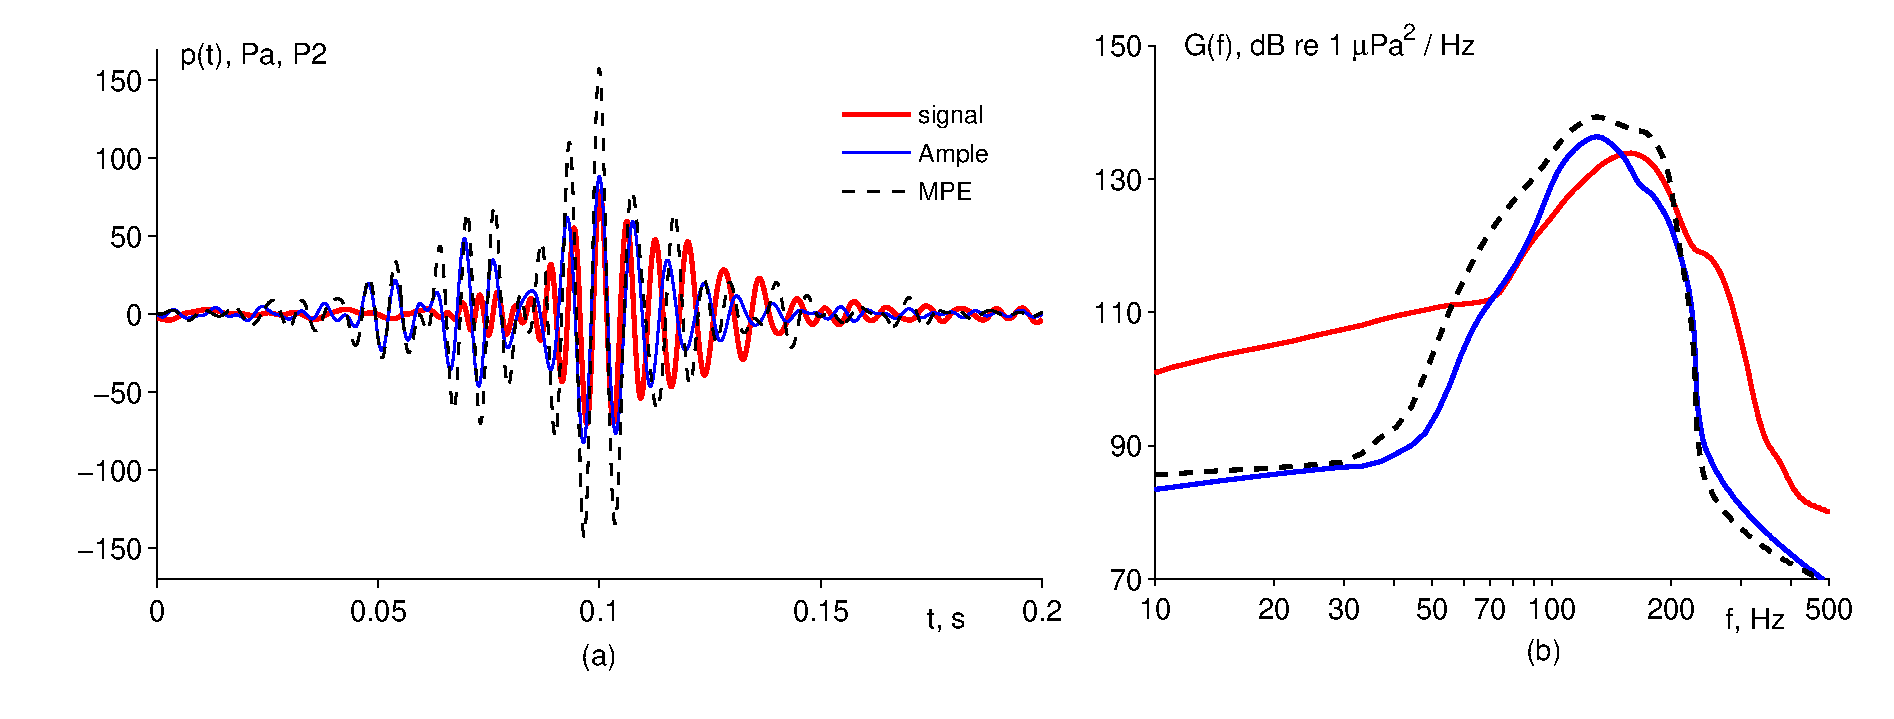
\includegraphics[width=0.9\textwidth]{seismo/pic_signal3.eps}
        \caption{Сравнение импульсных сигналов (\textbf{a}) и их спектров (\textbf{b}), полученные из данных измерений и результатов моделирования в точке наблюдения.}
        \label{fig::waveform_and_spectra}
    \end{figure}
    \FloatBarrier
    \newpage
    \par В \textbf{Заключении} приведены основные результаты работы:
    \begin{itemize}
        \item Разработана и апробирована методика численного решения псевдодифференциальных модовых параболических уравнений с искусственным ограничением расчётной области путём постановки граничных условий прозрачности или добавления к ней согласованных поглощающих слоёв.
        \item Разработан комплекс программ на языке программирования C++, который может быть использован для моделирования распространения тональных и импульсных сигналов, а также вычисления скалярных и векторных акустических полей антропогенных шумов в океане с возможностью учёта батиметрических и гидрологических данных, структуры слоёв дна, и ориентированный на максимальную производительность.
        \item Моделирование антропогенных шумов, связанных с сейсморазведочными работами и судоходством, проведённое с использованием разработанного комплекса прикладных программ, позволило добиться согласия уровней акустической экспозиции (SEL) с данными прямых измерений с точностью до 1 дБ и согласия значений распределения энергии в децидекадных частотных полосах на различных расстояниях от источника шума с точностью до 5 дБ для диапазона частот, в котором сосредоточена большая часть энергии сигнала.
    \end{itemize}
	\newpage
    \begin{refsegment}
        \printbibliography[title=Цитированная литература,notkeyword={myarticles},notkeyword={myproceedings},notkeyword={myprograms}]
    \end{refsegment}
    \begin{refsegment}
        \newrefcontext[labelprefix=A]
        \printbibliography[title=Список публикаций,filter=mine,resetnumbers=true]
    \end{refsegment}
    \newpage
    \thispagestyle{empty}
    \makeatletter
    ~
    \vskip 3cm
    \begin{center}
        \textit{Научное издание}\\
        \vspace{2cm}
        \@author\\
        \vspace{2cm}
        АВТОРЕФЕРАТ\\
        диссертации на соискание учёной степени\\
        кандидата физико-математических наук на тему:\\
        \@title
    \end{center}
    \vfill\null
    \begin{center}
        Подписано в печать \@FEFUdate[16.06]{6cm} \@FEFUpostfield{Заказ № }{128}{\widthof{Заказ № 9999}}\\
        Формат $60\times90\ 1/16$. Тираж 110 экз.
    \end{center}
    \begin{center}
        Отпечатано с авторского оригинал-макета в ТОИ ДВО РАН\\
        690041, Владивосток, ул. Балтийская, д. 43.
    \end{center}
    \makeatother
\end{document}
